\documentclass{standalone}
\usepackage{tikz}
\usepackage[]{xcolor}
\usetikzlibrary{calc}
\usepackage{bbold}
\usepackage{physics}

\newcommand{\mcG}{\mathcal{G}}

\graphicspath{{../figs/}{/home/jadeleon/Documents/doctorado/2025-2/protocolo_candidatura/gfx/chaos/}}


\usepackage{amsmath, amsthm, amssymb}
\colorlet{coscolor}{blue}

\newcommand{\red}{\color{red}}
\newcommand{\blue}{\color{blue}}
%Colors

\definecolor{max}{rgb}{1,0.54,0.1}
\definecolor{medium}{rgb}{1,0.8,0.6}
\definecolor{min}{rgb}{1,0.9,0.8}
\begin{document}
\pagestyle{empty}
\newcommand{\tmpa}{6}
\newcommand{\xo}{0.5}
\newcommand{\separation}{1.02}
\newcommand{\scalefont}{1}
%meanLevelSpacing_distribution_chaotic
\begin{tikzpicture}
\node[anchor=north west] at (\xo, 0) {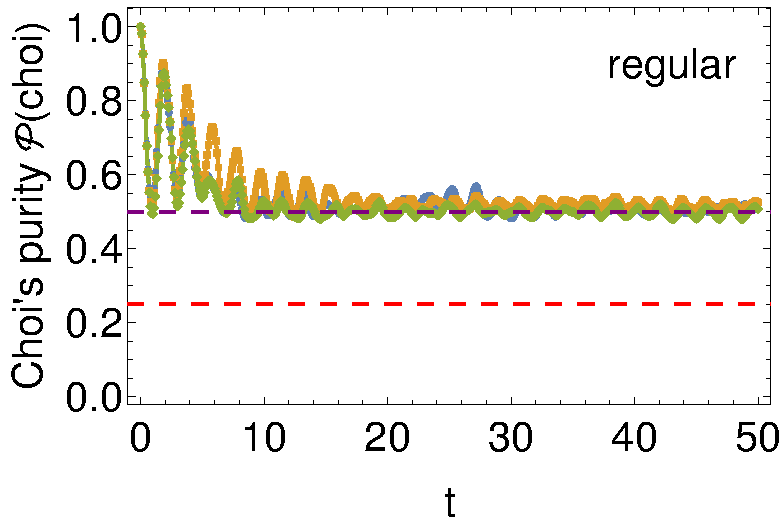
\includegraphics[width=\tmpa cm]{choi_regular_purity.pdf}};
\node[anchor=north west] at (\xo + \separation*\tmpa, 0)
{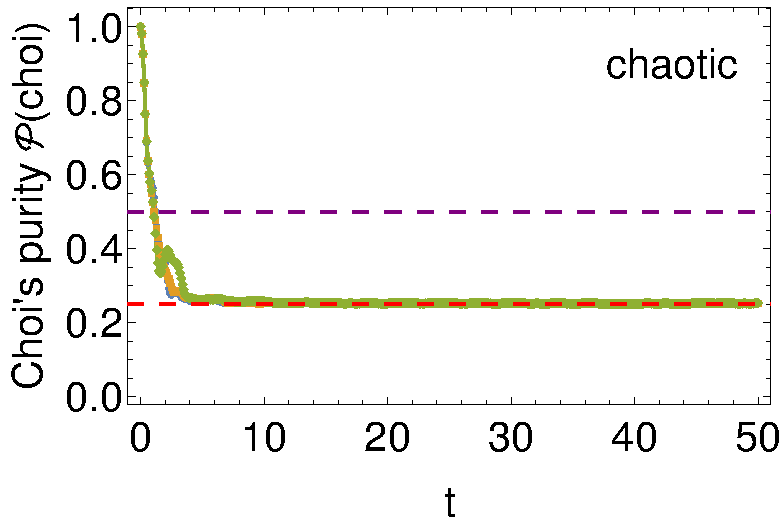
\includegraphics[width=\tmpa cm]{choi_chaotic_purity.pdf}};

\node[anchor=north west] at (\xo + 0.62*\separation*\tmpa, -0.15)
{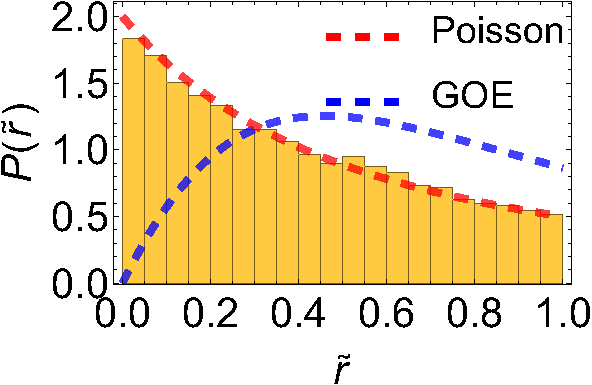
\includegraphics[height=1.33cm]{meanLevelSpacing_distribution_regular.pdf}};
\node[anchor=north west] at (\xo + 1.62*\separation*\tmpa, -0.15)
{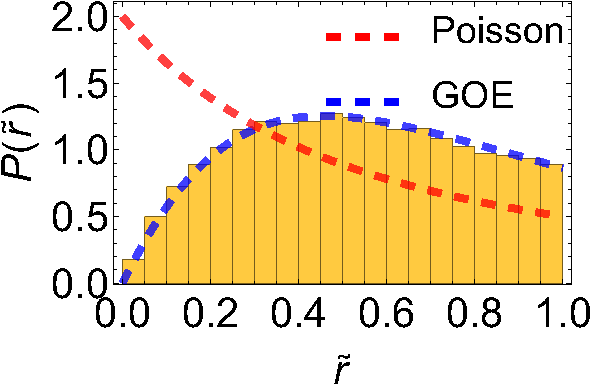
\includegraphics[height=1.33cm]{meanLevelSpacing_distribution_chaotic.pdf}};

\fill[white] (0.7, -4) rectangle (1.01, -0.2);
\node[rotate=90] at (0.85, -1.77) {$\Tr[\mathcal D^2(t)]$};
\fill[white] (6.8, -4) rectangle (7.15, -0.2);
\node[rotate=90] at (6.95, -1.77) {$\Tr[\mathcal D^2(t)]$};
\fill[white] (3, -4.09) rectangle (5, -3.85);
\node at (4, -3.9) {$t$};
\fill[white] (10, -4.09) rectangle (12, -3.85);
\node at (10.1, -3.9) {$t$};

\node[anchor=north west] at (1.75, -0.15) {\scalebox{\scalefont}{(a)}};
\node[anchor=north west] at (7.8, -0.15) {\scalebox{\scalefont}{(b)}};
\end{tikzpicture}
\end{document}